\documentclass[10pt, letterpaper]{article}
\usepackage{graphicx}
\usepackage[bottom=1.0in]{geometry}
\topmargin=-0.9in
\oddsidemargin -.3in
\evensidemargin -0.3in
\textwidth=7.0in
%\itemsep= -0.5in
%\parsep= -0.04in

\usepackage[cmex10]{amsmath}
\usepackage{multirow}



\author{Madhusudan Govindraju 39267182 }
\date{}
\begin{document}
\title{EEL5840  Elements of Machine Intelligence - HW 3}
\maketitle

The steps done to solve the assignment has been outlined in detail along with the assumptions and the data used.\\

The formula for LMS gradient descent algorithm used is as follows 

\begin{verbatim}
	for index=1:size(W)
         error = (X'* W - y);
         tempW(index) = W(index) + (mu) * error' * X(index);
	end
\end{verbatim}

and the formula used for Normalized LMS algorithm is 
\begin{verbatim}
	for index=1:size(W)
         error = (X'* W - y);
         tempW(index) = W(index) + (mu) * error' * X(index) /(X' * X);
	end
\end{verbatim}

The range for the order is from 1 to 100 and the range for the mu is chosen from 0.01 to 1 with 10 bins. \\

With this we first the gradient descent algorithm on the data available in v alidate.mat to get the surface plot shown in the figure . From this we obtain the order M and mu for which we obtain least MSE. We now save these as $M^{*}$ and $mu^{*}$. Which is the optimal order and step size. \\

We calculate the theoretical step size with the formula $$ mu = 1 / M*trace(R) $$ where $R$ is the eigen value matrix. If $|R| = 0$ then we can calculate with the formula $$ mu = 1/||X||$$ where $||X||$ is the norm of the signal. The practical step size should be approximately $0.10\times$theoretical step-size. 

\begin{enumerate}
\item With the above mentioned algorithm, we calculate the optimal values of the hyper parameters with the data in the validate.mat to get the optimal step size and optimal order of the filter design. From the implementation we get the optimal step size as $mu = 0.11$ and optimal order as $M=60$ . The figure 1 is a 3D dimensional plot of the MSE vs Step size and filter order. \\

\begin{figure}
\centering
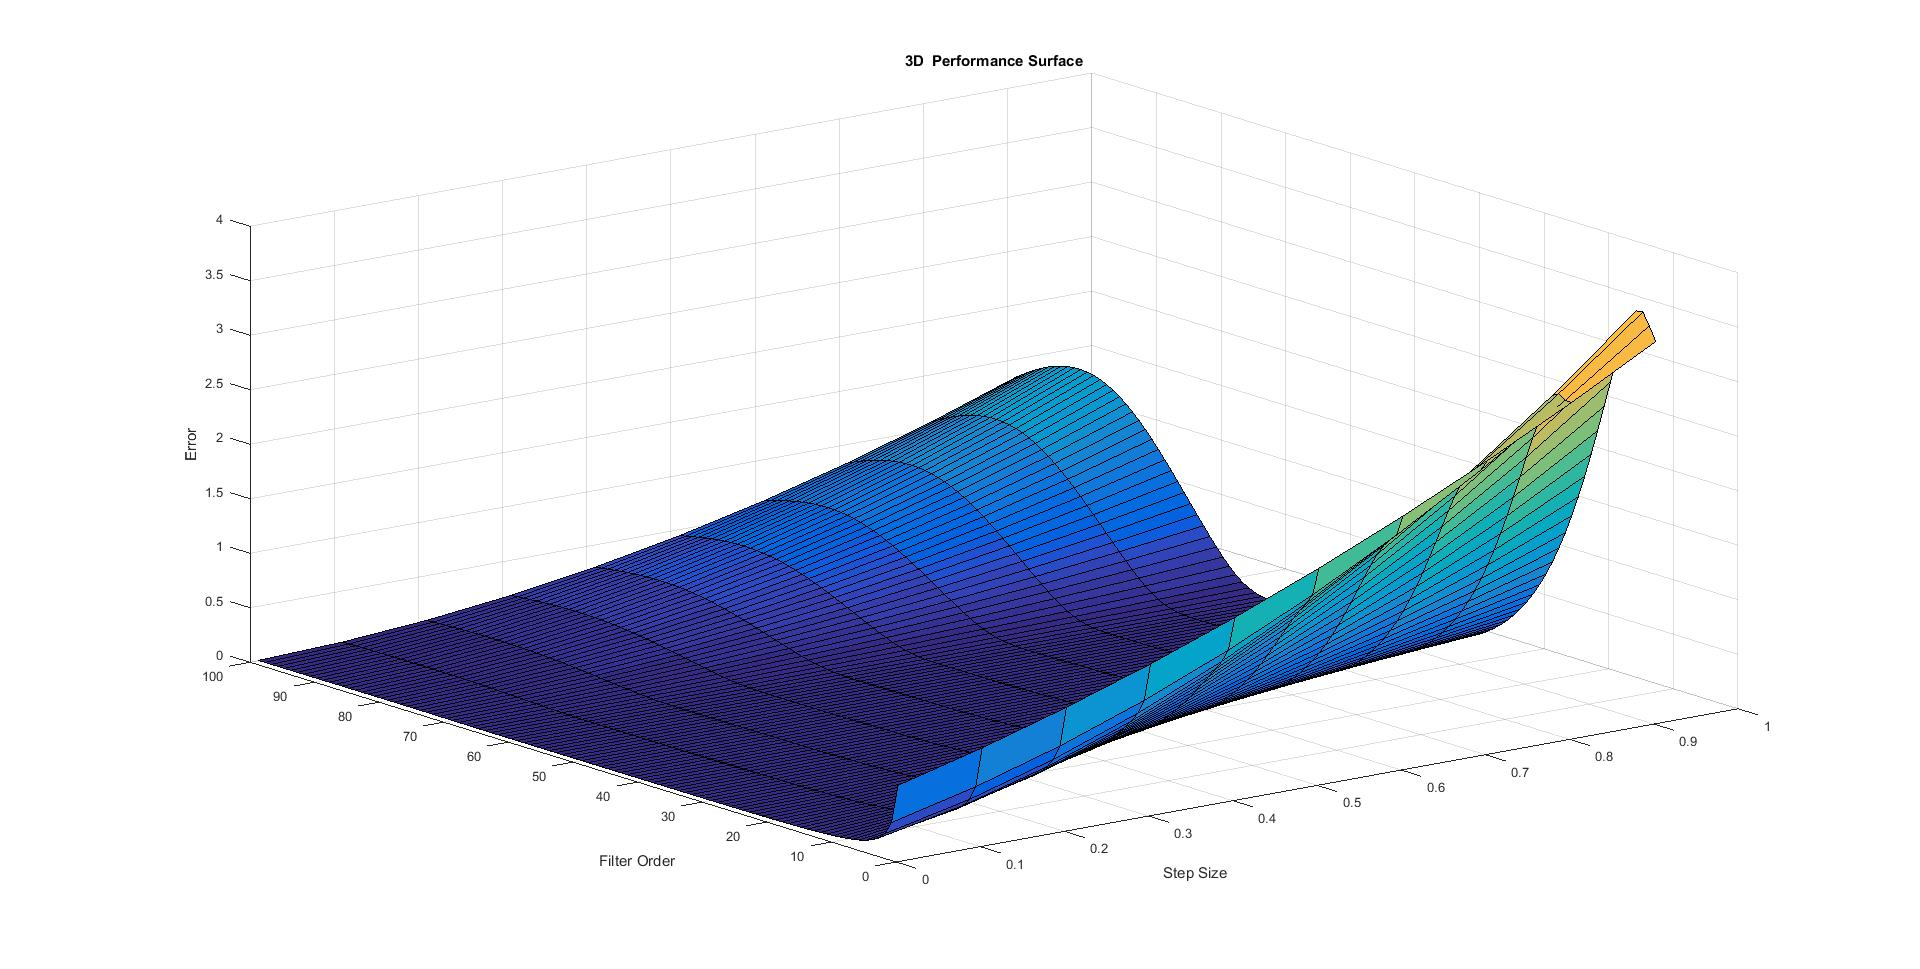
\includegraphics[scale=0.25]{3d_performanceSurface-Training.jpg}
\caption{3D Performance Surface plot}
\end{figure}

The theoretical step size has a formula  $ mu = 1 /M*trace(R) $ and $R$ is the auto correlation matrix, which is dependent on the input. The Input can be controlled with the filter order(M) hence the step size is related to the filter order . The step size should vary with the filter order, Also the condition for the system to be stable is $0<mu<1/\lambda_{max}$. This $\lambda_{max}$ is the eigen value of the Autocorrelation matrix, formed from the input hence this is another proof that the step size should be a factor of the signal order.

\item Now taking the best step size $mu=0.11$ and best order $M=60$ we plot the cost vs iteration to get the learning rate curve. This is available in the figure 2.  We take two other step sizes to understand how the learning rate changes with the step size. From the figure , we can understand that increasing the step size only ends with a cost which is higher than the optimal cost. But reaches the least cost sooner compared to the lower step sizes. Keeping a very low step size also reaches to the optimal cost. But it takes a longer time to reach this optimal cost. So choosing the optimal step size is important to achieve a good learning rate. 


\begin{figure}
\centering
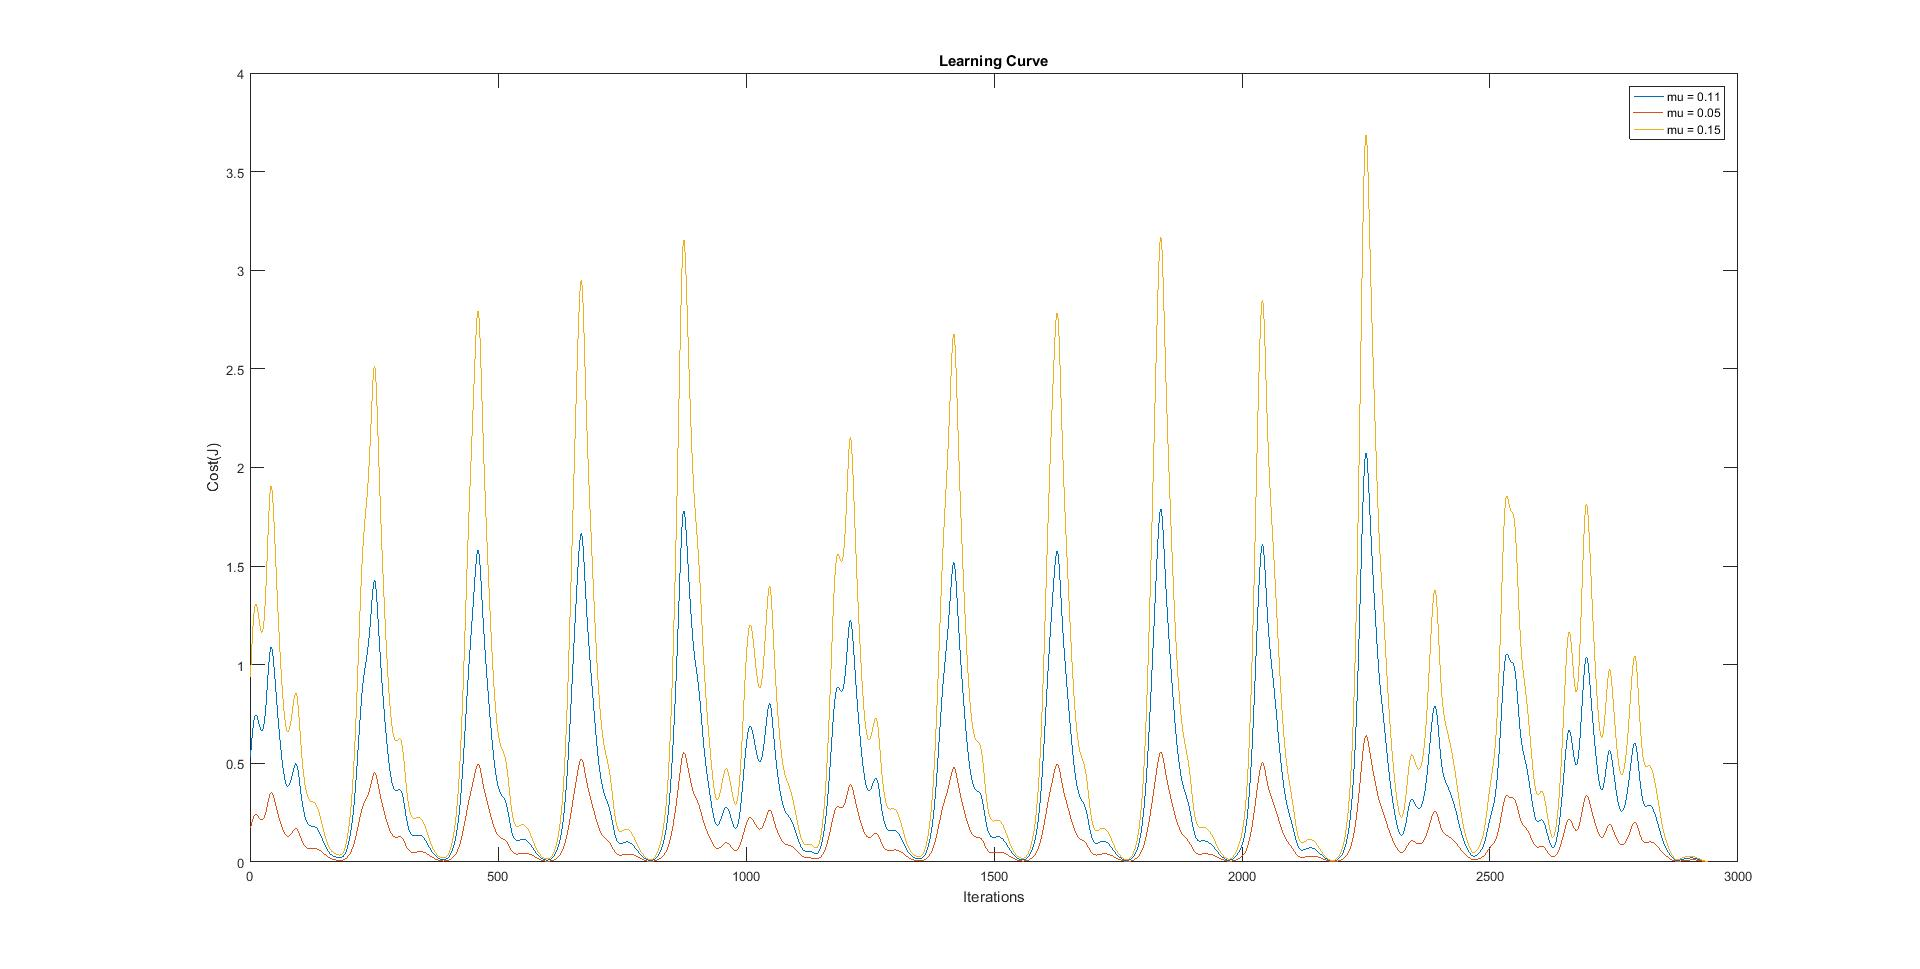
\includegraphics[scale=0.30]{Learning_Curve.jpg}
\caption{Learning Curve}
\end{figure}

The learning curve we obtain is very noisy because the fixed $mu$ leads to divergence in case the signal power changes. From the plot we can also see that choosing a lesser step size for the learning plot gives us lesser iterations but choosing a larger size leads to 

\item The main drawback of normal LMS algorithm is it i very hard to choose the learning rate $mu$ that guarantees the stability of the algorithm. $ 0<mu<1/\lambda_{max}$. So If the signal power changes, the fixed $mu$ can lead to divergence. This can be controlled by normalizing the step size with input power.
We repeat the steps in question one and two to obtain the best hyper parameters with the validation data and train it with the training data. Use that to predict the test.mat to obtain the performance. \\

For  the real world signals, we are using online processing, not batch processing hence the fixed mu is going to cause deviations which can be avoided using the normalised algorithm. Hence NLMS is better for real world signals.\\

For regression just taking into account the computational factor we can say that LMS is better as we dont have to calculate the $X'* X$. But for real world signals ,with the signals changing power it is better to have NLMS. 

\item From the implementation we can easily compare the computation required for the LMS and the linear adaptive system in HW2. In the linear adaptive filter system the computation $W = R^{-1}*P$ gives a computation complexity of $O(M^{2}*N)$. and additionally for the inverse we need a $M^{3}$ complexity using gaussian elimination, but in our case the $R$ matrix is a TOEPLITZ matrix and hence the inversion is only going to cost us a complexity of $O(M^{2})$. SO adding up all the complexities the complexity for the term $W = R^{-1}*P$ comes up to $O(M^{2}N) + O(MN) + O(M^{2}) $.  But in the computation for $W(n+1) = W(n) + \mu * Error * X(n)$ we have simple matrix multiplication with no autocorrelation or inverse computation hence we get the complexity equal to $O(N)$. Hence simplifying the equation by a number of times. So using the LMS is way more computationally efficient compared to the linear adaptive filter. Hence using LMS is more effective. 

\end{enumerate}



\end{document}